\section*{Web Appendix D}

In this appendix we illustrate the relationship between the fixed effects publication bias and \emph{p}-hacking models, discussed in Section 2.4, using an example. Recall the definition of the fixed effects one-sided discrete p-hacking model,
\[
f_{\textrm{ph}}(x\mid\theta,\sigma)=\sum_{j=1}^{J}\pi_{j}\phi_{[c_{j},\infty)}(x\mid\theta,\sigma^{2}).
\]
Consider this model with mixture probabilities and underlying standard
normal distribution. The components of the mixture together with the
\emph{p}-hacking model are displayed in Figure \ref{fig:p-hacking plots}
for $\pi=(0.4,0.2,0.4)$.

Using Proposition $1$, we can write the publication bias model as
\begin{eqnarray*}
f_{\textrm{pb}}(x\mid\theta,\sigma) & = & \sum_{j=1}^{J}\pi_{j}^{\star}\phi_{[c_{j},c_{j-1})}(x\mid\theta,\sigma^{2})
\end{eqnarray*}
where $\pi_{j}^{\star}$ are mixture probabilities that depend on
$\rho_{j}$. 

The publication bias and \emph{p}-hacking models are, in this case, equivalent. To illustrate, consider the fixed effects
\emph{p}-hacking model with $\pi=(0.4,0.2,0.4)$ and underlying standard
normal distribution. It is quite easy to verify that the \emph{p}-hacking
model is equivalent to the publication bias model with selection probabilities$\rho\approx(1,0.3,0.03)$
and $\pi^{\star}=(0.38,0.11,0.51)$. To see why, notice that we can
write
\[
\pi_{j}^{\star}=a_{j}^{\star}\sum_{i=j}^{J}\frac{\pi_{j}}{a_{j}}
\]
where $a_{j}=1-\Phi(c_{j},\theta,\sigma^{2})$ and $a_{j}^{\star}=\Phi(c_{j-1},\theta,\sigma^{2})-\Phi(c_{j},\theta,\sigma^{2})$.
The we can use the expressions for $\pi_{i}^{\star}$ of Proposition
$1$ to formulate and solve a linear system for $\rho$ in terms of
$\pi^{\star}$. 

In this particular case,
\begin{eqnarray*}
\pi_{3}^{\star} & = & \pi_{3}a_{3}^{\star}=0.4\cdot0.95=0.38,\\
\pi_{2}^{\star} & = & 0.025\cdot(\pi_{3}+\pi_{2}/0.05)=0.11,\\
\pi_{1}^{\star} & = & 0.025\cdot(\pi_{3}+\pi_{2}/0.05+\pi_{1}/0.025)=\pi_{1}+\pi_{2}^{\star}=0.51.
\end{eqnarray*}
The $\rho$s can be solved for numerically to obtain $\rho\approx(1,0.3,0.03)$,
see the $\mathtt{R}$ file $\texttt{translating.R}$ for more details.

\begin{figure}
\noindent \begin{centering}
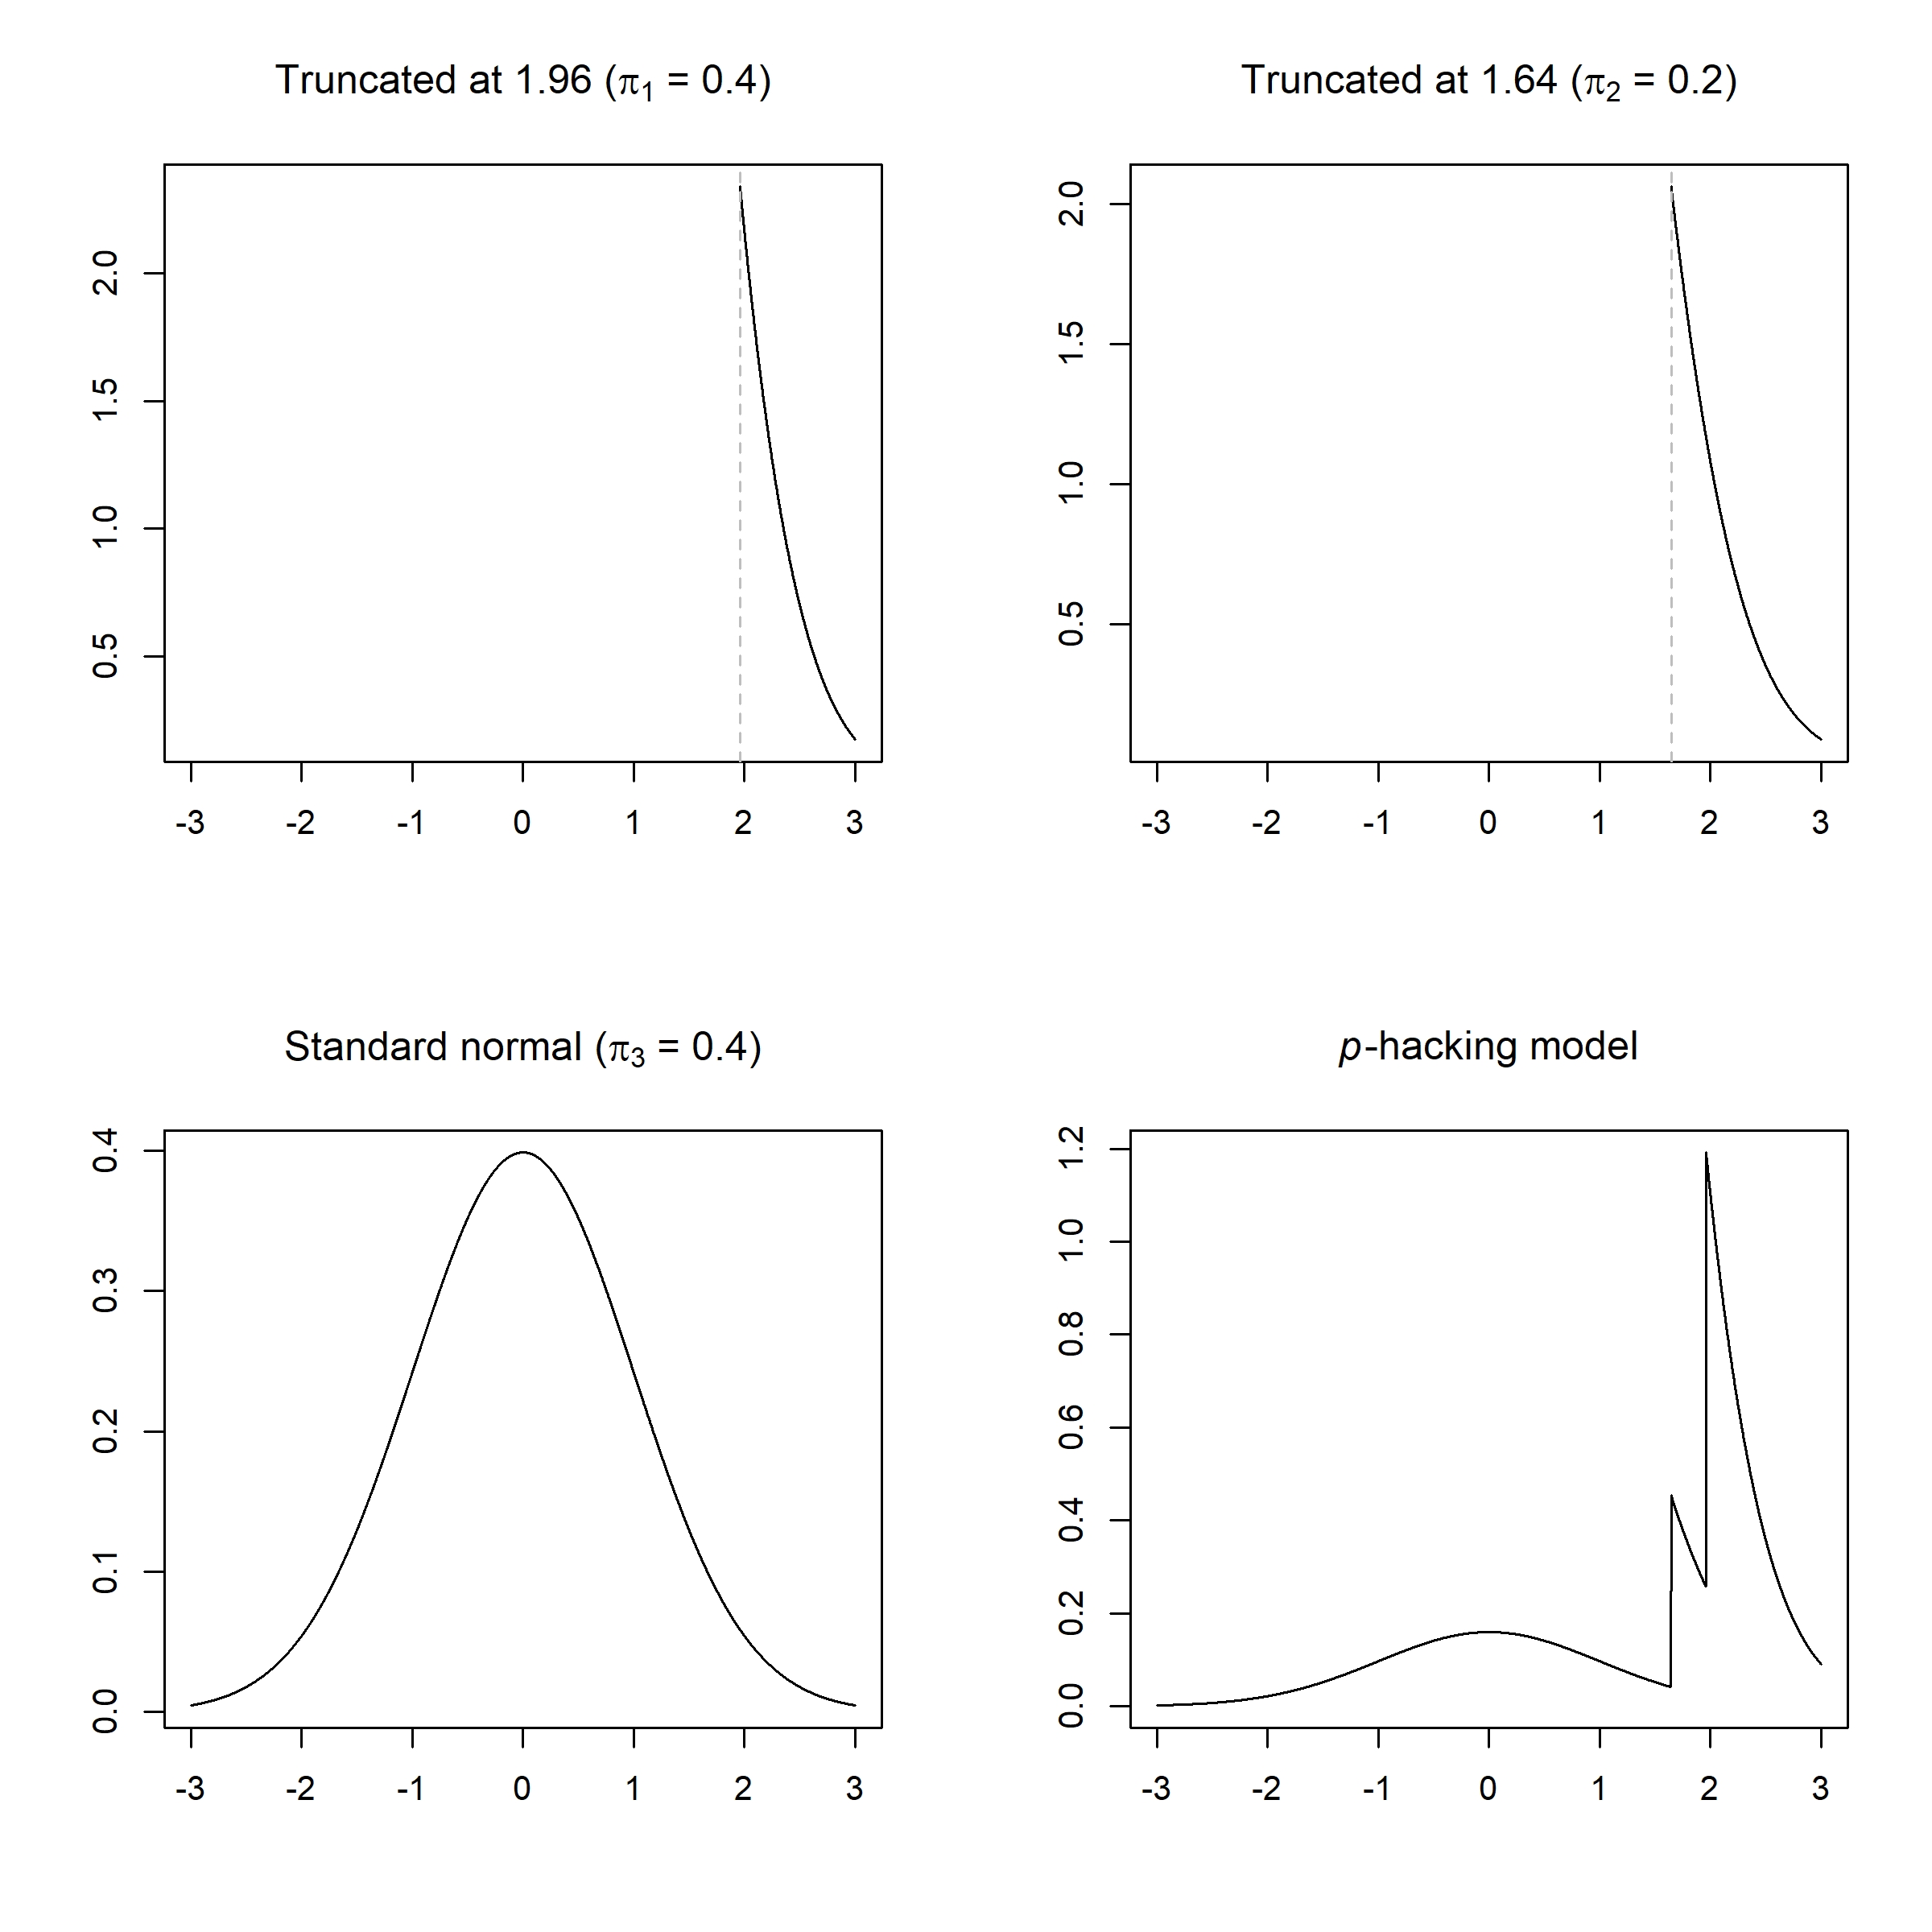
\includegraphics[scale=0.5]{plots/p-hacking}
\par\end{centering}
\caption{\label{fig:p-hacking plots}Illustration of the mixture components
of the \emph{p-}hacking model.}

\end{figure}

The publication bias model and the \emph{p}-hacking models are equivalent
under the fixed effects meta-analysis model, as formalized by the
following Lemma.
\begin{lem}
\label{lem:equivalence}Let $\{\sigma_{i}\}_{i=1}^{n}$ be
a collection of standard deviations and $\theta\in\mathbb{R}$ be
an underlying mean. Then there is a bijective function $g(\pi)=\pi^{\star}$
so that $\prod f_{\textrm{ph}}(x_{i}\mid\theta,\sigma_{i},\pi)=\prod f_{\textrm{pb}}(x_{i}\mid\theta,\sigma_{i},g(\pi))$
for any collection $\{x_{i}\}_{i=1}^{n}$ of observations.
\end{lem}

\begin{proof}
It suffices to show there is a bijective function function $g(\pi)=\pi^{\star}$
so that $f_{\textrm{ph}}(x_{i}\mid\theta,\sigma_{i},\pi)=f_{\textrm{pb}}(x_{i}\mid\theta,\sigma_{i},g(\pi))$
that is independent of $\sigma_{i}$. To do this, define $g(\pi)$
by $\pi_{j}^{\star}=a_{j}^{\star}\sum_{i=j}^{J}\frac{\pi_{j}}{a_{j}}$
to make a bijective function between $\pi$ and $\pi^{\star}$. Now
observe that both $a_{j}^{\star}$ and $a_{j}$ are independent of
$\sigma_{i}$ when $\theta$ is fixed. Thus $g(\pi)$ is independent
of $\sigma_{i}$ and the proof is done.
\end{proof}
You may use this lemma to transform the $\pi$s on the \emph{p}-hacking
form into $\pi^{\star}$ on the publication bias form and vice versa. 